\documentclass[11 pt]{llncs}
%\documentclass{sig-alternate}
% -------------defined commands------------
 \newcommand{\denom}{\empty}
 \newcommand{\suffix}{\empty}
 \newcommand{\suffixTwo}{\empty}
 \renewcommand{\suffix}{m,n}
 \newcommand{\suffixT}{1,1}
 
\newcommand{\PM}{\textit{PM}}
\newcommand{\LAP}{\textit{LAP}}
\newcommand{\EAP}{\textit{EAP}}
\newcommand{\TL}{\textit{TL}}
%
\newcommand{\userLabel}[1]{uLabel_{#1}}
\newcommand{\objectLabel}[1]{oLabel_{#1}}
%\newcommand{\UL}[1]{UL_#1}
%\newcommand{\OL}[1]{OL_#1}
%\newcommand{\userLabelOne}{$uLabel_1$}
%
%
%%---------EP-ABAC Models---------------%
\newcommand{\EPModels}{$EAP$-$ABAC$}
\newcommand{\EPZeroOneOne}{$EP_{0}$-$ABAC^{1,1}$}
\newcommand{\EPHOneOne}{$EP_{H}$-$ABAC^{1,1}$}
\newcommand{\EPSOneOne}{$EP_{S}$-$ABAC^{1,1}$}
\newcommand{\EPPMOneOne}{$EP_{\pm}$-$ABAC^{1,1}$}
\newcommand{\EPOneOneModels}{$EAP$-$ABAC_{1,1}$}
\newcommand{\EPMNModels}{$EP$-$ABAC^{m,n}$}
%
%\newcommand{\EPZeroOneOne}{\clabac}
%\newcommand{\EPHOneOne}{\hlabac}
%\newcommand{\EPSOneOne}{\slabac}
%\newcommand{\EPPMOneOne}{\npLabac}
%\newcommand{\EPOneOneModels}{$EAP$-$ABAC_{1,1}$}
\newcommand{\EPMNModel}{$EAP$-$ABAC_{m,n}$}
%
%
\newcommand{\LPModels}{$LAP$-$ABAC$}
\newcommand{\LPOneOne}{$LAP$-$ABAC_{1,1}$}
\newcommand{\LPMN}{$LAP$-$ABAC_{m,n}$}
\newcommand{\pmlabac}{$LaBAC_{\pm}^{1,1}$}
%
%% ---------------Other models-----------------
%\newcommand{\abacAlpha}{ABAC_\alpha}
%\newcommand{\hgabac}{$HGABAC$}
%\newcommand{\twoSortedRBAC}{2-sorted-RBAC}
%
%% ------------Higher Level LABAC---------------
%
%\newcommand{\labacOneTwoTwo}{$LaBAC_{1}^{2,2}$}
%\newcommand{\labacOneOneOne}{$LaBAC_{1}^{1,1}$}
%\newcommand{\labacOneMN}{$LaBAC_{1}^{m,n}$}
%\newcommand{\labacZeroMN}{$LaBAC_{0}^{m,n}$}
%\newcommand{\setLabac}{$LaBAC_{S}^{1,1}$}
%
%\newcommand{\labacNPMN}{$LaBAC_{\pm}^{m,n}$}
%\newcommand{\abacOneOne}{$LP$-$ABAC^{1,1}$}
%\newcommand{\labacOneOne}{$LaBAC^{1,1}$}
%
%%--------- LaBAC Names -----
%\newcommand{\labac}{$LaBAC$}
%\newcommand{\clabac}{$LaBAC_{0}^{1,1}$}
%\newcommand{\hlabac}{$LaBAC_{H}^{1,1}$}
%\newcommand{\slabac}{$LaBAC_{S}^{1,1}$}
%\newcommand{\npLabac}{$LaBAC_{\pm}^{1,1}$}
%\newcommand{\consLabac}{$LaBAC_{C}^{1,1}$}
%\newcommand{\elabac}{$LaBAC_{E}^{1,1}$}
%\newcommand{\labacOneOneFamily}{$LaBAC^{1,1}$}
%
%
%%------------LaBAC administrative ops-------------%
%\newcommand{\policyReview}{policy\_review}
%
%
%%-------------------- LaBAC Components-----------------
%\newcommand{\uLabel}{uLabel}
%\newcommand{\oLabel}{oLabel}
%\newcommand{\uLabelOne}{uLabel_1}
%\newcommand{\oLabelOne}{oLabel_1}
%\newcommand{\uLabelTwo}{uLabel_2}
%\newcommand{\oLabelTwo}{oLabel_2}
%\newcommand{\canAddPolicy}{can\_manage\_policy}
%\newcommand{\lb}{ }
%\newcommand{\OBJ}{O}
%\newcommand{\objmem}{o}
%\newcommand{\U}{U}
%\newcommand{\umem}{u}
%\newcommand{\amem}{a}
%\newcommand{\A}{A}
%
%\newcommand{\OLV}{OL}
%\newcommand{\olvmem}{ol}
%\newcommand{\ULV}{UL}
%\newcommand{\ulvmem}{ul}
%\newcommand{\OLA}{OLA}
%\newcommand{\ULA}{ULA}
%\newcommand{\OLH}{OLH}
%\newcommand{\ULH}{ULH}
%
%\newcommand{\policy}{Policy}
%\newcommand{\odominate}{\succeq_{ol}}
%\newcommand{\udominate}{\succeq_{ul}}
%\newcommand{\impliedPolicy}{Implied\_policy}
%\newcommand{\effectivePolicy}{Effective\_policy}
%\newcommand{\policyBound}{ValidPolicy}
%
%\newcommand{\maxPolicy}{|policy|_{max}}
%\newcommand{\maxPolicySet}{|\policy|_{max}}
%\newcommand{\request}{is\_authorized}
%
%
%% -------------session command------------
%\newcommand{\addSessionLabels}{add\_session\_labels}
%\newcommand{\removeSessionLabels}{remove\_session\_labels}
%\newcommand{\addSessionValues}{add\_session\_values}
%\newcommand{\removeSessionValues}{remove\_session\_values}
%\newcommand{\createSession}{create\_session}
%\newcommand{\deleteSession}{delete\_session}
%\newcommand{\createSubject}{create\_subject}
%\newcommand{\deleteSubject}{delete\_subject}
%\newcommand{\assignValues}{assign\_values}
%\newcommand{\removeValues}{remove\_values}
%
%%------------------ABAC^11 commands--------------
%
\newcommand{\UAV}[1]{\textit{UAV}_{#1}}
\newcommand{\OAV}[1]{\textit{OAV}_{#1}}
\newcommand{\ua}[1]{ua_{#1}}
\newcommand{\sa}[1]{sa_{#1}}
\newcommand{\oa}[1]{oa_{#1}}
\newcommand{\subCreator}{creator}
\newcommand{\uLabelP}[1]{\uLabel_{#1}}
\newcommand{\oLabelP}[1]{\oLabel_{#1}}
\newcommand{\ULS}[1]{ULS_{#1}}
\newcommand{\OLS}[1]{OLS_{#1}}
\newcommand{\val}[1]{\textit{Val}_{#1}}
\newcommand{\uVal}[1]{\textit{uVal}_{#1}}
\newcommand{\oVal}[1]{\textit{oVal}_{#1}}
\newcommand{\sessionLabelsP}[1]{\sessionLabels_{#1}}


%---------------ABAC, labac equivalence commands------------

\newcommand{\isAuthorized}{is\_authorized}
\newcommand{\GammaLabac}{\Gamma^{L}}
\newcommand{\gammaLabac}{\gamma^{L}}
\newcommand{\GammaA}{\Gamma^{A}}
\newcommand{\gammaA}{\gamma^{A}}
\newcommand{\GammaB}{\Gamma^{L}}
\newcommand{\gammaB}{\gamma^{L}}
\newcommand{\QLabac}{Q^{L}}
\newcommand{\qLabac}{q^{L}}
\newcommand{\QA}{Q^{A}}
\newcommand{\qA}{q^{A}}
\newcommand{\QB}{Q^{L}}
\newcommand{\qB}{q^{L}}
\newcommand{\qs}{q_s^{L}}
\newcommand{\qsa}{q_s^{A}}

\newcommand{\vdashA}{\vdash^{A}}
\newcommand{\vdashB}{\vdash^{L}}
\newcommand{\vdashLabac}{\vdash^{L}}
\newcommand{\GammaABAC}{\Gamma^{A}}
\newcommand{\gammaABAC}{\gamma^{A}}
\newcommand{\QABAC}{Q^{A}}
\newcommand{\qABAC}{q^{A}}
\newcommand{\vdashABAC}{\vdash^{A}}
\newcommand{\PABAC}{P^A}
\newcommand{\PLabac}{P^L}
\newcommand{\qal}{q_{aij}^L}
\newcommand{\qaa}{q_{aij}^A}
\newcommand{\ulpm}{UL_{\pm} }
\newcommand{\olpm}{OL_{\pm} }
\newcommand{\ulsubset}{UL_i}
\newcommand{\olsubset}{OL_j}
\newcommand{\gammaStartLabac}{\gamma_{0}^{L}}
\newcommand{\gammaStartABAC}{\gamma_{0}^{A}}
\newcommand{\gammaKLabac}{\gamma_{k}^{L}}
\newcommand{\gammaKABAC}{\gamma_{k}^{A}}

\newcommand{\mapping}{\overset{*}{\longmapsto_\psi}}
\newcommand{\mappingABAC}{\overset{*}{\longmapsto_{\psi_{A}}}}

%--------Tripli Commands ---------------
\newcommand{\mygamma}[2]{\gamma_{#1}^{#2}}
\newcommand{\myGamma}[1]{\Gamma^{#1}}
\newcommand{\mylongmapsto}[1]{\overset{*}{\longmapsto_#1}}
%\newcommand{\myVdash}{1}{\vdash^{#1}}
\newcommand{\myvdash}[1]{\vdash^{#1}}

\newcommand{\myq}[2]{q_{#1}^{#2}}
\newcommand{\myQ}[1]{Q^{#1}}
\newcommand{\myPSI}[1]{\Psi^{#1}}


%----------policy review functions---------


\newcommand{\subsetUL}{UL_s}
\newcommand{\subsetOL}{OL_s}
\newcommand{\setULs}{2^{UL}}
\newcommand{\setOLs}{2^{OL}}

%---------Tripli equivalence functions----------
\newcommand{\smallGamma}[1]{\gamma^{#1}}
\newcommand{\bigGamma}[1]{\Gamma^{#1}}
\newcommand{\smallQ}[1]{q_{s}^{#1}}
\newcommand{\bigQ}[1]{Q^{#1}}
\newcommand{\bigVdash}[1]{\vdash^{#1}}
\newcommand{\smallPsi}[1]{\psi^{#1}}
\newcommand{\bigPsi}[1]{\Psi^{#1}}

\newcommand{\curModelSymbol}{Z}
\newcommand{\manager}{mng}


\usepackage[utf8]{inputenc}
\usepackage{caption}
\usepackage{graphicx}
\usepackage{amsmath}
\usepackage{xcolor}
\usepackage{underscore}
\usepackage{epstopdf}
\epstopdfsetup{outdir=./}

\begin{document}

\pagenumbering{arabic}


%\title{On design and characterization of expressive powers of an enumerated policy finite domain ABAC model}
%\title{On design and analysis of expressive power of finite domain enumerated authorization policy ABAC models}
%\title{On Expressive Power of Enumerated Authorization Policy ABAC Models in Finite Domain}
%\title{On comparison of Finite Domain Logical-formula and Enumerated Authorization Policy ABAC Models in Expressive Power and Beyond}
%\title{On Expressive Power and Beyond of Logical-formula and Enumerated Authorization Policy ABAC Models in Finite Domain}
\title{A Comparison of Logical-formula and Enumerated Authorization Policy ABAC Models}


\date{30 July 1999}

\maketitle

\begin{abstract}
Attribute Based Access Control (ABAC) has gained considerable attention from businesses, academia and standards bodies (e.g. NIST  and NCCOE ) in recent years. ABAC uses attributes on users, objects and possibly other entities (e.g. context/environment), and specifies rules using these attributes to assert who can have which access permissions (e.g. read/write) on which objects.  Although ABAC concepts have been around for over two decades, there remains a lack of well-accepted ABAC models.  Recently there has been a resurgence of interest in ABAC due to continued dissatisfaction with the traditional models---notably Role Based Access Control (RBAC), Discretionary Access Control (DAC), and Lattice Based Access Control (LBAC).

There are two major techniques stated in the literature for specifying authorization policies in Attribute Based Access Control. The more conventional approach is to define policies by using logical formulas involving attribute values. The alternate technique for expressing policies is by enumeration. While considerable work has been done for the former approach, the later is comparatively less studied.  

%There remains many fundamental research problem to investigate, such as how to enumerate an authorization policy, how an enumerated authorization policy ABAC model should look like,  how enumerated policy is related to logical-formula policy and so on. 

In this dissertation, we conduct a systematic study of Enumerated Authorization Policy (EAP) for ABAC. We have developed a representative, simple EAP ABAC model---EAP-ABAC$^{1,1}$. For the sake of clarity and emphasis on different elements of the model, we present EAP-ABAC$^{1,1}$ as a family of models. We have investigated how the defined models are comparable to other existing EAP models. We also demonstrate capability of the defined models by configuring traditional LBAC and RBAC models in them. 

We compare theoretical expressive power of EAP based ABAC models to logical-formula authorization policy ABAC models. In this regard, we present a finite-attribute, finite-domain ABAC model for enumerated authorization policies and investigate its relationship with logical-formula authorization policy ABAC models in the finite domain. We show that these models (EAP-ABAC and LAP-ABAC) are equivalent in their theoretical expressive power. We respectively show that single and multi-attribute ABAC models are equally expressive.

As proof-of-concepts, we demonstrate how EAP ABAC models can be enforced in different application contexts. We have designed an enhanced EAP-ABAC$^{1,1}$ model to protect JSON documents. While most of the existing XML protection model consider only hierarchical structure of underlying data, we additionally identify two more inherent characteristics of data--- semantical association and scatteredness and consider them in the design. Finally, we have outlined how EAP-ABAC$^{1,1}$ can be used in OpenStack Swift to enhance its ``all/no access'' paradigm to ``policy-based selective access''.



\end{abstract}
\section{Introduction}

Access control has been a major component in enforcing security and privacy requirements of information and resources with respect to unauthorized access. While many access control models have been proposed only three, viz., DAC, MAC and RBAC, have received meaningful practical deployment. DAC (Discretionary Access Control) \cite{sandhu1994access} allows resource owners to retain control on their resources by specifying who can or cannot access certain resources. To address inherent limitations of DAC such as trojan horses, MAC (Mandatory Access Control) \cite{sandhu1994access}  has been proposed which mandates access to resources by pre-specified system policies. While both of these two models are based on fixed and predetermined policies, RBAC (Role Based Access Control) \cite{rbac} is a policy neutral, flexible and administrative friendly model.  Notably RBAC is capable of enforcing both DAC and MAC.  MAC is also commonly referred to as LBAC (Lattice-Based Access Control).

Attribute Based Access Control (ABAC) has gained considerable attention from businesses, academia and standard bodies (NIST \cite{nist-abac-draft} and NCCOE \cite{nccoe-abac-draft}) in recent years. ABAC uses attributes on users, objects and possibly other entities (e.g. context/environment) and specifies rules using these attributes to assert who can have which access permissions (e.g. read/write) on which objects.  Although ABAC concepts have been around for over two decades there remains a lack of well-accepted ABAC models.  Recently there has been a resurgence of interest in ABAC due to continued dissatisfaction with the three traditional models, particularly the limitations of RBAC.

%On the other hand, researchers and practitioners have long recognized essence of  attributes (user attributes, object attributes and context/environment attributes) in authentication and/or authorization decisions. For example, X.500 and X.509 \cite{xfiveonine}, LDAP \cite{ldap} or XACML \cite{xacml} are available for a long time which use attributes for either authentication or authorization decision. Some advantages of attributes in the authorization decision include following.

%Besides these models, researchers and practitioners have long recognized essence of  attributes (user attributes, object attributes and context/environment attributes) in authentication and/or authorization decisions. For example, X.500 and X.509 \cite{xfiveonine}, LDAP \cite{ldap} or XACML \cite{xacml} are familiar practitioner standard in this line available for a long time. The motivation of using attributes along with identities is long-standing. Attributes over identities are convenient in the following ways.

%\begin{itemize}
	%\item \emph{Hard to know user's real identity in a Open Environment: } In order to use identities, user's real identity has to be known beforehand. Often time, it is not possible to know the real identity of a user, specially when users come from a open environment like the Internet.
	
	%\item \emph{Hard to manage access control decision in large scale using Identity:} Using identities to specify access control decision, soon become infeasible when there are large number of users or objects to manage. On the other hand, as many users or objects can be specified using smaller set of attributes, they  are more preferable  in large distributed environment.
	
	%\item \emph{Anonymity or partial Identity:} Some times it is not required or even desirable to provide access control without knowing the real identity of a user. For example, in case of a digital library it may be enough to know some of the user attributes like membership or affiliation. On the other hand, for eligibility requirement of buying an alcoholic beverage, the age attribute may suffice without revealing the real identity.
	
	%\item \emph{Richer model for business function or logic in the authorization process:} Role, role hierarchy, role-based constraint easily capture some of the business function or logic of an organization related to role or job position in the organization. But in order to express business requirements in a more coherent way, it requires support for additional attributes.
	
%\end{itemize}



%Motivated by these requirements, various models have been proposed that accommodate attributes with traditional RBAC model \cite{rbac-with-attribute1, kuhn2010adding}. Another line of work is toward defining  a standalone model for Attribute Based Access Control (ABAC).

To demonstrate expressive power and flexibility, several ABAC models including  \cite{abacAlpha,hgabac,abac-for-web-service} have been proposed in past few years. These models adopt the conventional approach of designing attribute based rules/policies as logical formulas. Using logical formulas to grant or deny access is convenient because of the following reasons.

\begin{itemize}
	\item \emph{Simple and easy:} Creating a new rule for granting access is simple. It does not involve upfront cost like engineering roles in case of RBAC.
	
	\item \emph{Flexible:} Rules are easy to succinctly specify even complex policies. There is no limit on how many attributes can be used in a rule or how complex the language be to specify the rule. Given a required set of attributes, and a computational language, ABAC policy is only limited to what the language can express \cite{nist-abac-draft}.
\end{itemize}

Interestingly, designing a rich computational language to define attribute-based rules makes policy update or policy review an NP-complete or even undecidable problem. For example, authorization policies in many existing ABAC models including \cite{abacAlpha, hgabac, abac-for-web-service} are expressed  in propositional logic. Reviewing policy in these models (which may simply ask, for a given policy  which (attribute, value) pairs evaluate the policy to be true) is similar to the satisfiability problem in propositional logic which is NP-complete. Likewise review for policies specified in first-order logic is undecidable.

Another method for specifying attribute-based policies is by enumeration. Policy Machine \cite{policy-machine} and \twoSortedRBAC{} \cite{two-sorted-rbac} fall into this category. Enumerated policies  can also be very expressive. Ferraiolo et al \cite{policy-machine} show configuration of LBAC, DAC and RBAC in Policy Machine using enumerated policies.  Moreover, updating or reviewing an enumerated policy is inherently simple (polynomial time) because of its simple structure.  It should be noted that the size of an enumerated policy may be exponential relative to a succinct formula which expresses the same policy.  Thus there is a trade-off between these two methods for specifying policies.

In this paper, we present an ABAC model named Label-Based Access Control (LaBAC). In LaBAC, users are assigned a single label named $\uLabel$ and objects are assigned a single label named $\oLabel$. For a particular action, a policy in LaBAC is an enumeration using $\uLabel$ and $\oLabel$ values.

Labels ($\uLabel$ and $\oLabel$) in LaBAC are special types of attributes. While semantics of attributes in general are open-ended, labels have very specific semantics. For example, in general attributes can be set valued (e.g. roles) or atomic valued (e.g. age). Values of an attribute can be assigned by administrators (e.g. roles), derived from other attributes (e.g. membership type), self asserted (e.g. date of birth),  system specified (e.g. time) and so on. Moreover, values can be ordered or unordered.  On the other  hand, labels are specifically defined to be set valued, values are partially ordered and are only assigned by administrators. Intentionally, we use abstract names for labels---$\uLabel$ and $\oLabel$.  In an actual instance of LaBAC, labels can be given more appropriate names. For example, roles or clearance for $\uLabel$ and classification or sensitivity for $\oLabel$.

%In this paper, we represent LaBAC as a family of models---starting from the basic model, \clabac{} to the most advanced model, \labacOneOneOne{}.  In \hlabac{}, we add label hierarchies to \clabac{} while in \consLabac{} we add additional machinery to express constraints using labels. Finally, \labacOneOneOne{} combines all three models.

We analyze the expressive power of LaBAC with respect to other enumerative models. We also show that LaBAC can be viewed as a simple instance of Policy Machine (PM).  While, PM is more general and complex by covering other interesting aspects of access control, LaBAC is more scoped regarding development and progress towards ABAC models. On the other hand, we show equivalence of LaBAC and \twoSortedRBAC{} with respect to theoretical expressive power. Finally, we show flexibility of LaBAC by configuring traditional models (LBAC \cite{lbac} and RBAC\cite{rbac}) in it.

Rest of the paper is organized as follows. In Section \ref{sec:background}, we briefly discuss logic-based policy and enumerated policy along with a review of related literature. Section \ref{sec:model} presents a family of LaBAC models. We show the equivalence of LaBAC and \twoSortedRBAC{} in Section \ref{sec:equivalence}. Section \ref{sec:configuration} presents configuration of tradition RBAC and LBAC policy in LaBAC. We express LaBAC as a simple instance of Policy Machine in Section \ref{sec:pm}. Finally, Section \ref{sec:conclusion} concludes the paper.

%   which adopts the enumerated style for expressing authorization policies. LaBAC can  be viewed as a simple instance of Policy Machine (PM). LaBAC uses one user attribute ($\uLabel$) and one object attribute ($\oLabel$) and a authorization policy in LaBAC for an action is an enumeration using these two attributes. 

\section{Authorization policy representation}

\label{sec:background}
In this section, we discuss two types of authorization policies - logical-formula and enumerated policy wrt finite domain attributes based on the assumption of the finiteness of attribute values. 
\subsubsection{Finite domain ABAC}
%\textbf{Finite domain ABAC model}
	\section{Assumption of Finite Domains}
\subsection{Finite policies for Finite domain ABAC}

\textbf{Theorm 1:} \\
For L boolean variables at most $2^{2^L}$ distinct boolean expression can be defined over logical AND, OR and NOT operators. 

\textbf{Theorm 2:} \\
Let UA be the set of user attributes, OA be the set of object attributes and $A=UA \cup OA$. For an attribute $a \in A$, let $R(a)$ denote co-domain or range of the attribute. Further $OPS$ be the set of all comparison operators that compares user/object attribute with other attribute values or constant values. The maximum number of boolean variable (expression of the form (value op value) ) that can be defined comparing attribute values are $|A| \times |OP| \times \sum_{a \in A} R(a)$
	%\subsection{Enumerated \& logical-formula authorization policy}

\vspace{-.5em}
%\textbf{Logical-formula authorization policy}
\subsubsection{Logical-formula authorization policy}
Logical-formula authorization policy (\LAP{}) can be defined as a boolean expression consisting of subexpressions connected with logical operators (for example, $\land, \lor, \lnot$ and so on ) where each subexpression compares attribute values with other attribute or constant values. The language for \LAP{} usually supports a large set of logical and relational operators. A \LAP{} grants a user request for exercising certain action on an object if attributes of the requesting user and requested object evaluate the formula true. $Auth_{read} \equiv clearance(u) \succeq classification(o)$ is an example of  logical-formula authorization policy which allows a user to read an object if the user's clearance dominates classification of the object.

\LAP{}s are usually expressed in propositional logic. Examples of  \LPModels{} models  include \cite{abacAlpha,hgabac,abac-ws,abac-for-web-service}.  Flexibility of these models have been demonstrated by configuring conventional DAC\cite{dac}, MAC\cite{lbac} and RBAC \cite{rbac} policies in it. It has been shown  \cite{labac} that policy review in  \LPModels{} is equivalent to the satisfiability problem  which is NP-complete for propositional logic. 
\vspace{-1em}
%in proposition logic (or in first-order logic if LAPs are expressed in it) which makes the complexity of reviewing policies NP-complete in \LPModels{} models.


%\textbf{Enumerated authorization policy}
\subsubsection{Enumerated authorization policy}
	An enumerated authorization policy (\EAP{}) consists of a set of  tuples.  Each tuple \textit{(UAVals, OAVals)} grants privileges to a set of users  to exercise an action on a set of objects identified by the user and object attribute values \textit{UAVals} and \textit{OAVals} respectively. In an EAP, each tuple is distinct and grants privileges independently. Both  UAVals{} and OAVals{} can be atomic valued or set valued. (\textit{\manager, TS}) and (\textit{\{\manager, dir\}, \{TS,H\}}) are example of atomic and set valued tuples respectively. 
	
Usefulness of \EAP{}s have been demonstrated in the literature. For example, \textit{Policy Machine (PM)} \cite{policy-machine} and \labac{} \cite{labac} show flexibility of \EAP{}s by their ability to configure traditional models. 


%For example, in Policy Machine (PM) \cite{policy-machine}, Ferraiolo et. al define attribute based enumerated policies using one user attribute, one object attribute and a set of actions. PM also shows how to configure traditional models including DAC \cite{dac}, MAC \cite{lbac}, RBAC \cite{rbac} and Chinese wall \cite{chinese-wall}  using enumerated policies \cite{INCITS526}. On the other hand, \labac{} is another example showing usefulness of enumerated policies. A comparative analysis of enumerated authorization policy and logical-formula authorization policy is discussed in Section \ref{sec:LP-vs-EP}






%\subsection{Tripli Experssive power}


	
	
 	\begin{figure} 
 		\centering
 		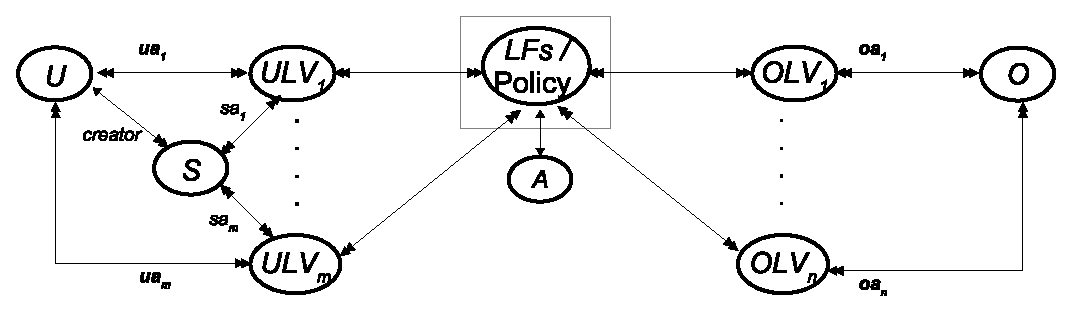
\includegraphics[width=.9\textwidth]{DBSEC16/lpabac-mn}
 		\caption{Components of \LPModels{} model with m user and n object attributes}
 		\label{fig:lp-abacmn-diagram}
 	\end{figure}
	
	
	\label{sec:models}
	%In this section, we define a multi-attribute enumerated authorization policy ABAC model named \EPMNModel{} (shown in Figure \ref{fig:epabac-mn}). To the best of our knowledge, \EPMNModel{} is the first such model. \PM{}\cite{policy-machine} also defines a multi-attribute \EPModels{} model, but their interpretation of attributes is different than the traditional interpretation of \textit{(attribute-name, value)} pairs. 
	
	Here we define a multi-attribute \LPModels{} model named \LPMN{} (shown in Figure \ref{fig:lp-abacmn-diagram})  by abstracting its policy language and potentially accepting any computational logic as policy language. While existing \LPModels{} models  define their own policy language, \LPMN{} can subsume any policy language which further generalizes our equivalence results presented in the following section.  The differences between \EPMNModel{} and \LPMN{} are highlighted in boxes in the figures. 
	


		%\vspace{-1em}
\begin{table}[t]
	\centering
	\caption{ \LPMN{} model} %\vspace*{3pt}
	\label{tab:lp-abacmn-definition}
		\begin{tabular}{|l|}						
		\hline					
				\multicolumn{1}{|c|}{\underline{\textit{I. Sets and relations}}}\\			
				 - $U, O$, $S, A$ (set of users,  objects , subjects and actions resp.)\\
				 %- $ \UAV, \textit{\OAV}$ and $A$ (finite set of user and object attribute values and actions resp.) \\
				 - $\UAV{1}, \UAV{2}, ..., \UAV{m}$ (range of user attribute functions) \\
				 - $\OAV{1}, \OAV{2}, ..., \OAV{n}$ (range of object attribute functions) \\
				 - $UA = \{\ua{1}, \ua{2}, ..., \ua{m}\}$ (set of all user attributes);   $\ua{i}: U \to 2^{\UAV{i}}$ for $1 \le i \le m$\\
 				 -  $OA = \{\oa{1}, \oa{2}, ..., \oa{n}\}$ (set of all object attributes); $\oa{i}: O \to 2^{\OAV{i}}$ for $1 \le i \le n$\\
  			     - $\creator: S \to U$, many-to-one mapping \\
 				 - $SA = \{\sa{1}, \sa{2}, ..., \sa{m}\}$ (set of all subject attributes); $\sa{i}(s) \subseteq \ua{i}(\creator(s))$\\	
				
				%$\langle$ see Table \ref{tab:abac11-session} for user level session functions $\rangle$ \\
				
				 \multicolumn{1}{|c|}{\underline{\textit{II. Policy components}}} \\						
				
				-  $f_a: (2^{\UAV{1}}, 2^{\UAV{2}}, ... ,2^{\UAV{m}}, 2^{\OAV{1}},  2^{\OAV{2}}, ... , 2^{\OAV{n}} )\to \{true, false\}$ (policy for $a \in A$).  \\
   			    - $LFs = \{f_a | a \in A \} $ ( set of all policies)\\			
				 
				
				 \multicolumn{1}{|c|}{\underline{\textit{III. Authorization function}}} \\						
				- \request(s:S,\amem:A,\objmem:O) = \\	\hfill  $\exists f_a \in LFs[f_a(\sa{1}(s), \sa{2}(s),..., \sa{m}(s),  \oa{1}(o), \oa{2}(o), ... \oa{n}(o)) = true] $  
			
\\ \hline	
	\end{tabular}
	
\end{table}

%\vspace{-1em}


	
	
	
	


%\subsubsection{\LPMN{} - a multi-attribute logical-formula authorization policy ABAC model.}
	\label{sec:lpmodels}
	 
	  
 	\begin{figure} 
 		\centering
 		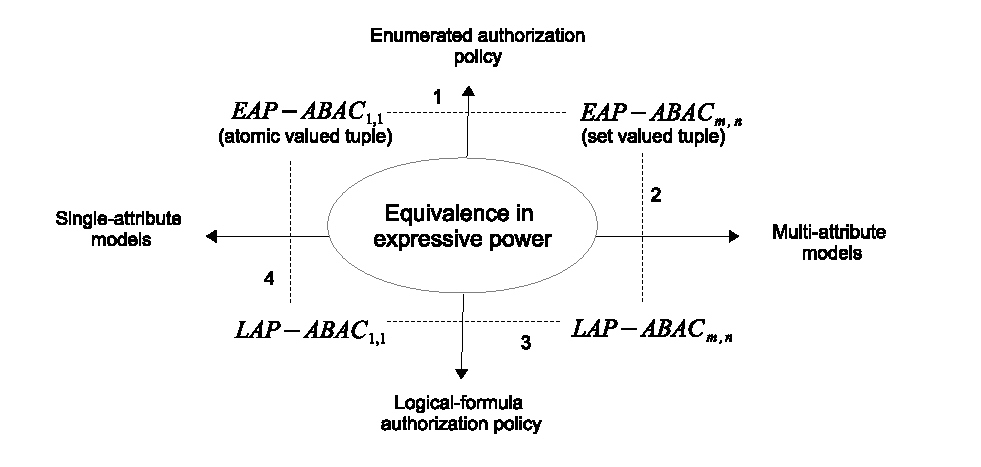
\includegraphics[width=.9\textwidth]{DBSEC16/all-equivalence}
 		\caption{Equilavence of enumerated and logical-formula auth. policy ABAC models}
 		\label{fig:all-equivalence}
 	\end{figure}
 

	 \LPMN{} (given in Figure \ref{fig:lp-abacmn-diagram}) is very similar to \EPMNModel{}, except it is based on LAPs.  It has an unbounded set of users, objects and sessions and a finite set of user attributes, object attributes, session attributes and authorization policies. \LPMN{} does not define an concrete policy language. Instead, it defines  authorization policies as any boolean function that takes values of $m$ subject and $n$ object attributes as parameters. If attribute values of a requesting subject, and requested object evaluate the authorization function $f_a$ (defined for action $a \in A$) true, corresponding access is granted. The formal definition of the model is given in Table \ref{tab:lp-abacmn-definition}. We deliberately maintain similar sets and relations (compare to \EPMNModel{})  to assert that these models only differ in the definition of authorization policies. 
	 

	

\chapter{EAP-ABAC vs LAP-ABAC in expressive power}
\label{sec:beyond}
In practice, usefulness of an access control system depends on many other aspects beyond its expressive power. For example, in the NIST special publication \textit{Guidelines  for Access Control System Evaluation Metrics} \cite{access-control-evaluation}, the authors divide these aspects into four categories including (i) administration, (ii) enforcement, (iii) performance and (iv) support. In this section, we mostly focus on administrative properties. We compare the aforementioned models from two perspectives---single-attribute vs multi-attribute and enumerated vs logical-formula authorization policy.

\subsection{Single Attribute vs Multiple Attributes}

We have seen earlier that \EPOneOneModels{} is equivalent to \EPMNModel{} and \LPOneOne{} is equivalent to \LPMN{}. But, in practice this may not be useful because of many reasons including the following.

\textbf{Attribute-value assignments and administration.} Ranges of each attribute intrinsically separate their values. For example, if \textit{role} and \textit{location} are two different attributes, values of these attributes are inherently distinguished. As a result, attribute-value assignments to users and objects and administration of these values (add or remove existing values) can be separated using semantics of individual attributes.

\textbf{Privacy concern.} If we combine values of  more than one attribute into single attribute values, a user may expose more credential than required in a particular context.  For example, combining values \textit{role} and \textit{location}, we may create values \{\textit{manager@campus, manager@home}\}. If so, a user cannot hide role  when the context requires only his location.


\newcommand{\office}{\text{office}}
% \newcommand{\highlight}[1]{%
% 	\colorbox{black!19}{$\displaystyle#1$}}
 
\begin{table}
	\centering
	\caption{ Different representations of  $Auth_{read}$ policy  ($Auth_{read}$ states that \textit{\manager} can access \textit{TS} objects  from either \textit{office} or \textit{home} locations)} 
	\label{tab:LAP-heterogeneity}
	\begin{tabular}{|l|}						
		\hline					
			
			(i) $  \manager \in role(u) \land (\office{} \in location(u) \highlight {\lor home \in location(u)})  \land TS \in sensitivity(o)$ \\
			(ii) $((\manager \in role(u) \land \office{} \in location(u) ) \highlight {\lor (\manager \in role(u) \land home \in location(u) )}  )$ \\ \hfill $ \land TS \in sensitivity(o)$\\
			(iii) $((\manager \in role(u) \land \office{} \in location(u) \land TS \in sensitivity(o) ) \highlight{\lor}$  \\ \hfill $\highlight{((\manager \in role(u) \land home \in location(u) \land TS \in sensitivity(o) )}$ \\
		 \hline	
	\end{tabular}	

	
\end{table}


\textbf{Larger set to manage.} Combining values of more than one attribute together, we often need to manage larger set of values. For example, if there are ten possible values of \textit{role} and ten possible values of \textit{location}, by combining them we may need to manage one hundred values.  



\subsection{Enumerated vs Logical-Formula Authorization Policy}
In this section, we consider pros and cons of logical-formula and enumerated   authorization policy. Usually, logical formula   allows us powerful language constructs to formulate even complicated business logic and policies in a succinct way. Logical formulas often support large number of logical and relational operators which make it easy to set up new policies. On the downside,  logical formulas impose little constraint on the structure, size or style of the authorization policy. As a result, policies are heterogeneous in nature having different sizes and styles. Even a single policy can be represented in so many ways.  For example, Table \ref{tab:LAP-heterogeneity} shows how a policy $Auth_{read}$ can  be represented in three different  forms. The heterogeneity across multiple policies and lack of a canonical form make it difficult to understand, update or administer existing policies.  For example, to update $Auth_{read}$ so that \textit{manager} no longer gets access from \textit{home}, different representations of the policy need to be updated in different ways. Required changes to policies are highlighted in Table \ref{tab:LAP-heterogeneity}. These changes require  manual effort  by an administrator to update them. In a different aspect, LAPs are often monolithic, making it difficult to distinguish sub-policies.




On the other hand, enumerated authorization policies (EAPs), have a distinct form of representation. Thus, in \EPModels{} models, policies are homogeneous and  sub-policies in a policy can be presented in one or more tuples, and a  policy is a set of such tuples. Different tuples are distinguishable from each other and can be thought of as micro-policies. Thus, policies in enumerated tuples are polylithic as opposed to monolithic in logical formula. 

%Usefulness of micro policies is further discussed in Section \ref{sec:usefulness}.

On the flip side, an EAP can be very large as it  does not allow conditional expressions. For example, the  condition \textit{$age(u) \ge 18$}, should be achieved by enumerating all possible ages greater or equal 18. Another disadvantage  is that when we add/remove attributes from the system, existing EAPs may require to be updated. 

\vspace{-1em}

\subsubsection{Administration Using Micro-Policies}
\label{sec:usefulness}

The policy $Auth_{read}$ mentioned above can be represented using micro-policies as $\{( \{\manager\}, \{\office\},$ $ \{TS\} )$, $( \{\manager\}, \{home\}, \{TS\} )\}$. In order to update the policy so that \textit{manager} can no longer access from \textit{home}, we can remove the second tuple resulting $Auth_{read} \equiv \{( \{\manager\}, \{\office\}, \{TS\} )\}$. Similarly, we can add new micro-policies adding new tuples to $Auth_{read}$.

Thus, in term of administration, the minimum administrative units in EAP are micro-policies represented by policy tuples. So, it is possible that an EAP can be managed by multiple administrators at the most fine grained level of micro-policies. Design of an administrative model to manage micro-policies is beyond the scope of this dissertation. We postulate that as policy update can be done by merely adding or removing policy tuples,  it can be done programmatically  in \EPModels{} model. Figure \ref{fig:policy-pros-cons} shows pros and cons of \EPModels{} and \LPModels{} models. Table \ref{tab:pros-cons-table} presents a detailed comparison.




\vspace{-1em}


%\subsubsection{Canonicalization of Enumerated Authorization Policy}

%In this section, we show how we can represent EAPs in a canonical form. Consider, $Auth_{write} \equiv \{( \{\manager\}, \{TS\} )$, $ ( \{\manager, dir\}, \{TS\} )\}$ in $EP$-$ABAC_{1,1}$. The first tuple says someone who is at least manager (can additionally have any other roles) can write \textit{TS} objects. The second tuple says someone both manager \& director (may additionally have any other roles) can write \textit{TS} objects. Thus, the first tuple also includes authorization requirements of the second tuple. So, if we update $Auth_{write}$ to remove the second tuple,  effectively updated $Auth'_{write}$ also represents the old policy. Thus, an enumerated authorization  policy can be represented in more than one ways which violates uniqueness of the canonical form. The advantage of representing policies in canonical form is that we make sure by adding or removing tuples, we really update the policy.  This would help  in the automation of policy administration. 


% It authorizes a \textit{manager } to access \textit{TS} objects from  \textit{office}. If the same \textit{manager} additionally holds a \textit{director} role, $Auth_{read}$ also authorizes him. This is because the authorization function checks if the requester at least (not exactly) possesses the values specified in the tuple.  Thus, if  we update $Auth_{read}$ to add a new tuple $(\{manager, director\}, \{office\}, \{TS\})$, the updated policy semantically represents the same old policy. (because the new tuple is subsumed by another tuple in the policy). Thus, an EAP can be represented in more than one forms which violets uniqueness of canonical form. 


 	\begin{figure} 
 		\centering
 		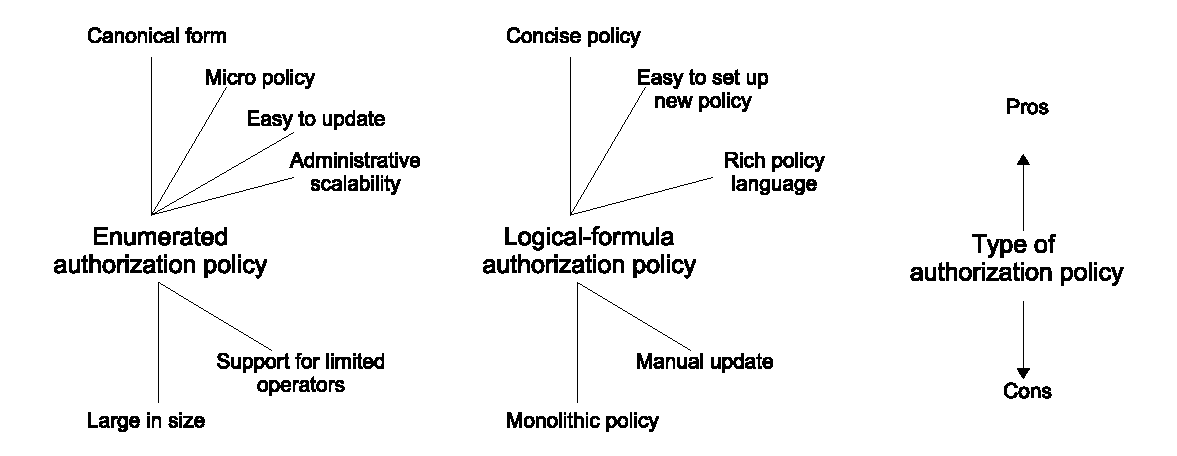
\includegraphics[width=.9\textwidth]{DBSEC16/policy-pros-cons}
 		\caption{Pros and cons of enumerated and logical-formula authorization policy}
 		\label{fig:policy-pros-cons}
 	\end{figure}

\begin{table}[]
\centering
\caption{Comparison of  LAP  and  EAP }
\label{tab:pros-cons-table}
\begin{tabular}{|c|c|c|}
	\hline
Characteristics    of   &  \begin{tabular}[c]{@{}l@{}} LAPs  (considering \\ $ABAC_\alpha$/HGABAC)  \end{tabular}     & \begin{tabular}[c]{@{}l@{}}  EAPs  (value enumeration \\ for  positive attribute-values) \end{tabular}        \\ \hline
\multicolumn{3}{l}{} \\ 
\multicolumn{3}{l}{\textit{\textbf{Definition}}} \\ \hline
\begin{tabular}[c]{@{}l@{}} \textit{distinguishing features}\end{tabular} & \begin{tabular}[c]{@{}l@{}}  logical-formula \end{tabular} & \begin{tabular}[c]{@{}l@{}}  enumeration\end{tabular} \\ \hline
\multicolumn{3}{l}{} \\ 
\multicolumn{3}{l}{\textit{\textbf{Syntax}}} \\ \hline

\begin{tabular}[c]{@{}l@{}}\textit{Representation} \end{tabular} & \begin{tabular}[c]{@{}l@{}} expression \end{tabular} & \begin{tabular}[c]{@{}l@{}} set  \end{tabular} \\ \hline

\begin{tabular}[c]{@{}l@{}}\textit{Morphism} \end{tabular} & \begin{tabular}[c]{@{}l@{}} polymorphic (single policy can \\  be represented many ways) \end{tabular} & \begin{tabular}[c]{@{}l@{}} unique representation \end{tabular} \\ \hline

\begin{tabular}[c]{@{}l@{}}\textit{Policy type}\end{tabular} & \begin{tabular}[c]{@{}l@{}} macro-policy, \\ possibly cohesive sub-policies\end{tabular} & \begin{tabular}[c]{@{}l@{}} micro-policy, \\ disjointed sub-policies  \end{tabular} \\ \hline

\begin{tabular}[c]{@{}l@{}}\textit{Divisibility}\end{tabular} & \begin{tabular}[c]{@{}l@{}} monolithic\end{tabular} & \begin{tabular}[c]{@{}l@{}} polylithic  \end{tabular} \\ \hline


\begin{tabular}[c]{@{}l@{}}\textit{Size}\end{tabular} & \begin{tabular}[c]{@{}l@{}} usually concise\end{tabular} & \begin{tabular}[c]{@{}l@{}}  usually large  \end{tabular} \\ \hline

\begin{tabular}[c]{@{}l@{}}\textit{Language}\end{tabular} & \begin{tabular}[c]{@{}l@{}} propositional/ \\ first-order logic formula\end{tabular} & \begin{tabular}[c]{@{}l@{}} equivalent to DNF \\  of logical formula  \end{tabular} \\ \hline

 
 \multicolumn{3}{l}{} \\ 
 \multicolumn{3}{l}{\textit{\textbf{Semantics}}} \\ \hline
 
 \begin{tabular}[l]{@{}l@{}}\textit{Set of granted  privileges} \end{tabular} & \begin{tabular}[c]{@{}l@{}} dynamic (may change on addition/ \\removal  of attribute-values)\end{tabular} & \begin{tabular}[c]{@{}l@{}}static (privilege is explicitly\\ granted) \end{tabular} \\ \hline 


 \begin{tabular}[c]{@{}l@{}}\textit{Required attribute-value }\\ \textit{assgnments for granting} \\ \textit{privileges} \end{tabular} & \begin{tabular}[c]{@{}l@{}} partial assignments may \\  grant privilege\end{tabular} & \begin{tabular}[c]{@{}l@{}} requires complete assignment  \end{tabular} \\ \hline 
 
% \begin{tabular}[c]{@{}l@{}}\textit{ Privilege abstraction} \end{tabular} & \begin{tabular}[c]{@{}l@{}} may abstract granted privileges\end{tabular} & \begin{tabular}[c]{@{}l@{}} no privilege abstraction  \end{tabular} \\ \hline 

\multicolumn{3}{l}{} \\ 
\multicolumn{3}{l}{\textit{\textbf{Administration}}} \\ \hline

\begin{tabular}[c]{@{}l@{}}\textit{Cost of reviewing policy} \end{tabular} & \begin{tabular}[c]{@{}l@{}} NP-complete \end{tabular} & \begin{tabular}[c]{@{}l@{}} polynomial \\ (in number of tuples) \end{tabular} \\ \hline

%\multicolumn{3}{l}{\textit{\textbf{Privilege administration}}} \\ \hline

\begin{tabular}[c]{@{}l@{}}\textit{Granting new privilege} \end{tabular} & \begin{tabular}[c]{@{}l@{}} manual update \end{tabular} & \begin{tabular}[c]{@{}l@{}} add new tuples \end{tabular} \\ \hline

\begin{tabular}[c]{@{}l@{}}\textit{Remove existing privileges} \end{tabular} & \begin{tabular}[c]{@{}l@{}}manual update  \end{tabular} & \begin{tabular}[c]{@{}l@{}} remove tuples \end{tabular} \\ \hline 

\begin{tabular}[c]{@{}l@{}}\textit{Minimum administrative unit} \end{tabular} & \begin{tabular}[c]{@{}l@{}} entire policy \end{tabular} & \begin{tabular}[c]{@{}l@{}} micro-policy \end{tabular} \\ \hline   

\begin{tabular}[c]{@{}l@{}}\textit{scalability} \end{tabular} & \begin{tabular}[c]{@{}l@{}} not scalable  \end{tabular} & \begin{tabular}[c]{@{}l@{}} \hfil scalable \end{tabular} \\ \hline     

\multicolumn{3}{l}{} \\ 
\multicolumn{3}{l}{\textit{\textbf{Application}}} \\ \hline

\begin{tabular}[l]{@{}l@{}}\textit{} Convenient for \end{tabular} & \begin{tabular}[c]{@{}l@{}} specifying new policy, \\  administration using range \\ of attribute-values\end{tabular} & \begin{tabular}[c]{@{}l@{}}  updating policy, \\ fine grained administration\end{tabular} \\ \hline 

\begin{tabular}[l]{@{}l@{}}\textit{} Suitable environment \end{tabular} & \begin{tabular}[c]{@{}l@{}} open, loosely administered system, \\ distributed administration\end{tabular} & \begin{tabular}[c]{@{}l@{}}  close, tightly administered \\ system\end{tabular} \\ \hline 

                                        
\end{tabular}
\end{table}

%To represent \EAP{}s in a canonical form, we ensure that in the same policy, no policy-tuple subsumes another policy-tuple. Formally, let $t_i$ denotes $i^{th}$ tuple in a policy and $S_{ik}$  be the $k^{th}$ set in tuple $t_i$. We say, a policy tuple $t_i$ subsumes $t_j$ iff  $(\exists p \in \{1,2,..,m+n\}, \forall q \in \{1,2,..,m+n\} \setminus {p})[S_{ip} \subseteq S_{jp} \land (S_{iq} \subseteq S_{jq} \lor S_{ip} = S_{jp}) ]$. For example, for $t1=(\{\manager,dir\}, \{TS\})$,$t2=(\{\manager, dir, adv\}, \{TS\})$, $t3=(\{\manager,dir, adv\}, \{H\})$ t1 includes t2 but none of t1 and t2 includes t3. 



%To maintain a canonical representation of EAPs, we can remove policy-tuples that have been subsumed by other tuples. It is also possible to specify more sophisticated meta policies to manage subsumed policy-tuples.  




\section{Related work}
\label{sec:related-work}
	%\subsection{Related work}

	Several attribute based access control models have been proposed in the literature. Most of them are based on logical-formula authorization policies. For example,	$\abacAlpha{}$ \cite{abacAlpha} is among the first few models to formally define an ABAC model.  $\abacAlpha{}$ was developed  for the specific purpose of simulating simple forms of DAC, MAC and RBAC policies. As such, it deliberately has a more restrictive (and less powerful) policy language.  On the other hand, $\hgabac{}$ \cite{hgabac} is more general in purpose and also capable of accommodating  the traditional models. Both $\abacAlpha{}$ and \hgabac{} use propositional logic as their policy language. In the very same direction, ABAC-for-web-services \cite{abac-for-web-service} is among very few earlier works to outline authorization architecture and policy formulation for an ABAC system. Other notable work for the development of logical formula ABAC model include \cite{grid-abac,ontologies,abac-ws,wang2004logic}.
	
    NIST ABAC guide \cite{nist-abac-draft} and other publications \cite{hu2015attribute}  are also significant in defining concepts, required components, considerations and architecture for designing an  enterprise ABAC system. They acknowledge the fact that ABAC rules can be quite complex in boolean combination of attributes or in simple relations involving attributes.    
    
%    It is designed to demonstrate flexibilities of an ABAC system to configure DAC, MAC and RBAC models. As such,
    
	%In the other direction, Policy Machine (PM) \cite{policy-machine} and \labac{} \cite{labac} are	examples of ABAC models based on enumerated authorization policy. A policy/privilege in PM is defined as $(ua_i, OP, oa_i)$, where $ua_i$ and $oa_i$ are values of user-attribute and object-attribute respectively and $OP$ is  a set of operations. A policy tuple in \labac{} is also defined a very similar way specified as $(user\_attr\_value, action, object\_attr\_value)$. Both of these two models have also demonstrate their flexibility in configuring traditional models in it. In a very similar way, authorization policies is enumerated in \twoSortedRBAC{} \cite{two-sorted-rbac} in the  context of role.  
	
	Damiani et al \cite{damiani2005} describe an informal framework for 	attribute based access control in open environments. Bonatti et al \cite{bonatti,bonatti2} present a uniform structure to logically formulate and reason about both service access and information disclosure constraints according to related entity attributes. 	
	
	Other related work include XACML \cite{xacml}, UCON \cite{ucon}, policy mining \cite{mining},attribute certificates \cite{attribute-cert} and so on \cite{enforcing,lee,foley}.
	
	 %ABE \cite{abe} 
	%Similarly, [28,29,30] develop a service negotiation framework for requesters and providers to gradually expose their attributes.

	 %XACML \cite{xacml} is a declarative access control policy language and processing model which  supports attribute based concepts and policies. Although, it lacks a formal definition of an ABAC model, it is notable for its uses in multiple commercial products.
	 

\section{Conclusion \& Future work}
\label{sec:conclusion}


In this paper, we present a simple Attribute Based Access Control model (LaBAC) using enumerated policies. LaBAC is based on single user attribute ($\uLabel$) and single object attribute ($\oLabel$). We analyze LaBAC with other enumerated policy models. LaBAC can be viewed as a simple instance of an existing enumerated policy model - Policy Machine. LaBAC is also equivalent to \twoSortedRBAC{}, which is the other enumerated policy model as we are aware of. We show flexibility of LaBAC in terms of configuring traditional models (RBAC and LBAC) in it. 

Besides enumerated policy, we also discuss logical formula based authorization policy which is the more conventional approach for designing ABAC policy.  Logical formula can be very rich and complex and capable of expressing even complicated business logic in a very succinct form. But policy review or policy update may become NP-complete in policies expressed in logical formulas. 
%We believe, reviewing or updating policy would be  crucial in maintaining an ABAC system. This motivates us to explore other avenues in the design of an ABAC model. 

Enumerated policies as an alternate to specify authorization policies raise many interesting issues that need to be addressed to better  understand the nature of ABAC. For example, are there other alternates to specify authorization policies or policies in general in a ABAC system? What are the pros and cons of using logical formula or enumerated policy? Does review of policy or policy update become any simple in enumerated policies?  

Additionally, many other questions need to be addressed in term of enumerated policy ABAC models. Are enumerated policy models as expressive (or less/more) as logical formula based models? How (if possible) can we express arbitrary business logic in enumerated policies? What would be the cost of storing potentially large number of enumerated tuples? How can we extend LaBAC to incorporate more than one user and object labels (or attributes) and so on?

%On the contrary, enumerated policy is simple and policy review in it is inherently polynomial time. But there are many issues we need to be addressed in term of enumerated policy model. Is enumerated policy model less (or equal/more) expressive in general than logical formula based model?  Is there a  trade-off between expressive power and complexity of policy review/policy update? What would be the cost of storing potentially large number of enumerated polices? Are there alternates of designing ABAC policy other than or in between two extremes of logical formula and enumerated tuples and so on. 
%%\vspace{-1em}
\renewcommand{\suffix}{m,n}
\newcommand{\suffixT}{1,1}
\begin{table}
	\centering
	\caption{ Mappings } %\vspace*{3pt}
	\label{tab:lp11-to-lpmn}
	\begin{tabular}{|l|}						
		\hline					
%			\multicolumn{1}{|c|}{\underline{\textit{I. \LPOneOne{} components}}} \\
%				  - $U, O, A, S, UAV, OAV$  (users,  objects, actions, subjects, user and object attr. values.)\\
%				  - $ua,oa$ (attribute functions);  $ua:U\to 2^{UAV}$; $oa:O\to 2^{OAV}$ \\ 
%				  - $\subCreator: S \to U$ ; $sa:S\to 2^{UAV}$,    $sa(s) \subseteq ua(\subCreator(s))$\\
%				  - $f_a: (sa(u), oa(o)) \to \{true, false\}$  and $\isAuthorized(s,a,o) =(f_a(sa(u),oa(o))=true$) \\
				 
		   
		   \multicolumn{1}{|c|}{\underline{\textit{I. From \LPMN{} to \LPOneOne{}}}}\\	
			   - $U = U_{\suffix}; O = O_{\suffix}; A = A_{\suffix}; S = S_{\suffix};$$\textit{UAV} = \UAV{1} \times \UAV{2}\times ... \times \UAV{m}$\\
			   -  $\textit{OAV} = \OAV{1} \times \OAV{2}\times ... \times \OAV{m}$;$ua(u) = \ua{1}(u) \times \ua{2}(u) \times ... \times \ua{m}(u) $\\
			   -$oa(u) = \oa{1}(u) \times  ... \times \oa{m}(u) $$sa(u) = \sa{1}(u) \times ... \times \sa{m}(u) $; $\creator(s) = \creator_{\suffix}(s)$\\
			    - $ f_a =$ $\mathop{\bigvee}\limits_{ f_{a_{m,n}}( \ULS{1}, \ULS{2},...\ULS{m}, \OLS{1}, \OLS{2}, ...,\OLS{n})=true }  (\ULS{1}(u) \times ... \times \ULS{m}(u) \subseteq ua(u) )\land$ \\ \hfill  $(\OLS{1}(o) \times ... \times \OLS{n}(o) \subseteq oa(o))$, for $\ULS{i} \subseteq \UAV{i}$ and $\OLS{i} \subseteq \OAV{i}$ \\ 		
			   
 
	   \multicolumn{1}{|c|}{\underline{\textit{II. From \LPOneOne{} to \LPMN{}}}}\\	
			- $U = U_{\suffixT}; O = O_{\suffixT}; A = A_{\suffixT}; S = S_{\suffixT};$\\
			- $\UAV{1} = UAV; \UAV{2} = \{\}; ... \UAV{m} = \{\};$  $\OAV{1} = OAV; \OAV{2} = \{\}; ... \OAV{n} = \{\};$\\
			- $\ua{1}(u) = ua(u); \ua{2}(u) = \{\};...\ua{m}(u) = \{\}$; $\oa{1}(o) = oa(o); \oa{2}(o) = \{\};...\oa{m}(o) = \{\}$\\
		    - $\sa{1}(u) = sa(u); \sa{2}(u) = \{\};...\sa{m}(u) = \{\}$; $\creator_{\suffix}(s) = \creator(s)$ and $f_{a_{\suffix}} =$\\
		    $\mathop{\bigvee}\limits_{ f_{a}( \ULS{i},\OLS{i})=true }  (\ULS{i} \subseteq \ua{1}(u) \land$   $ \OLS{i}\subseteq oa(o))$  for $\ULS{i} \subseteq UAV$ and $\OLS{i} \subseteq OAV$ \\ 
		 %\hline	
		 	\multicolumn{1}{|c|}{\underline{\textit{III. From \EPOneOneModels{} to \LPOneOne{} }}}\\					
		 	- $U  = U ; O  = O ; A  = A $; $UAV	= UL; OAV = OL$;$ua(u) = uLabel(u)$; $oa(o)=oLabel(o) $\\
		 	-  $sa(s) = \sessionLabels(s) $ ;$f_a =$ $\mathop{\vee}\limits_{ (ul_i, ol_i) \in \policy_a} ( ul_i \in ua(u) \land ol_i \in oa(o))$. \\
		 	
		 	\multicolumn{1}{|c|}{\underline{\textit{IV. From \LPOneOne{} to \EPOneOneModels{}}}}\\	
		 	- $UL= 2^{ULV}; OL= 2^{OLV}; \uLabel(u) = 2^{ua(u)};\oLabel(o) = 2^{oa(o)}; \sessionLabels(s) = 2^{sa(s)}$ \\	  
		 	- $\Policy_a = \{  (\ulsubset, \olsubset) | (\exists \ulsubset \subseteq UL, \exists \olsubset \subseteq OL)[ f_a(\ulsubset, o\ulsubset) = true] \} $
		 	
		 	\\ \hline	
	\end{tabular}	

	
\end{table}
%\vspace{-1.5em}












%%\vspace{-1em}
\renewcommand{\denom}{0}
\renewcommand{\suffix}{0}
\renewcommand{\suffixTwo}{0}
\begin{table}
	\centering
	\caption{ Mapping from \clabac{} to \EPMNModel{}  } %\vspace*{3pt}
	\label{tab:mapping-clabac-to-slabac}
	\begin{tabular}{|l|}						
		\hline					
			\multicolumn{1}{|c|}{\underline{\textit{I. \clabac{} components}}} \\
			-  $U_\suffix, O_\suffix,  A_\suffix, S_\suffix, UL_\suffix$, $OL_\suffix$ (users, objects, actions, sessions, $uLabel$ and $oLabel$ values resp.) \\ 				  
			-  $\uLabel_\suffix: U_\suffix \to 2^{UL_\suffix}$, $\oLabel_\suffix: O_\suffix \to 2^{OL_\suffix}$; $\creator_\suffix: S_\suffix \to U_\suffix$; $\sessionLabels_\suffix: S_\suffix \to 2^{UL_\suffix}$ \\
			- $\Policy_a \subseteq 2^{UL_\suffix} \times 2^{OL_\suffix}$ and $\Policy_\suffix = \{Policy_a | a \in A\}$\\
		   
	 \multicolumn{1}{|c|}{\underline{\textit{II. Construction}}}\\	
			- $U = U_\denom, O = O_\denom, A = A_\denom, S_\suffixTwo = S$ \\
			- $\UL{1} = \UL{0}$, $\UL{i} = \{\}$, for $2\le i \le m$\\
			- $\OL{1} = \OL{0}$, $\OL{i} = \{\}$, for $2\le i \le n$\\
			- $\uLabelP{1}(u) = \uLabelP{0}(u)$, $\uLabelP{i}(u) = \{\}$, for $2 \le i  \le m $\\
			- $\oLabelP{1}(o) = \oLabelP{0}(u)$, $\oLabelP{i}(o) = \{\}$, for $2 \le i  \le n $\\
			- $\creator_0(s) = \creator(s)$, for $s \in S$\\
			- $\sessionLabelsP{1}(s) = \sessionLabelsP{0}(s)$, $\sessionLabelsP{i}(s) = \{\}$, for $2 \le i \le m$\\
			- $\Policy_a = \{( \{ul\}, \{\}, ...\{\}, \{ol\}, \{\}, ... \{\} ) | (ul,ol) \in \Policy_a[ \Policy_a \in \Policy_\suffix]\}$\\
		 \hline	
	\end{tabular}	

	
\end{table}
%\vspace{-1em}
We acknowledge an error found in the authorization function of the  \EPMNModel{} model as found in Table 1  of 4th page of this paper. The updated definition of the authorization function (with corrections highlighted) is presented below. \\

$is\_authorized(s:S, a:A, o:O) = (\exists (ULS_1,ULS_2, ..., ULS_m, OLS_1,$ \\$ OLS_2, ... OLS_n ) $ 
$ \in Policy_a)[ULS_i \highlight{=} sLabel_i(s), \text{for } 1 \le i \le m \land$  \\ \hfill $ \OLS{i} \highlight{=} oLabel{i}(o), \text{for } 1 \le i \le n]$ 

\bibliographystyle{abbrv}
\bibliography{sigproc}
\vspace{-2em}


\end{document}
